\section*{Exploration numérique}
\phantomsection
\addcontentsline{toc}{section}{Exploration numérique}

\subsection*{Question 1 — départ en état 2}
\phantomsection
\addcontentsline{toc}{subsection}{Question 1 — départ en état 2}
Nous allons calculer \(\Pi^{(n)} = \Pi^{(0)} M^{n}\) avec \(\Pi^{(0)} = e_2\) (vecteur unité en position 2 pour commencer à l'état 2) et \(M\) la matrice 27\(\times\)27 fournie.
Nous allons utiliser le programme réalisé en projet de C \texttt{markov\_analyzer} \parencite{markovGraphAnalyzer2025} qui va  reconstruire d'abord la matrice de transition \(M\) à partir du fichier fourni sur Moodle, puis calculer les distributions \(\Pi^{(n)}\) pour \(n=1,2,10,50\).
\begin{itemize}[label=\textbullet]
  \item Arguments utilisés : \\
  \texttt{./markov\_analyzer -{}-in data/moodle/matrix.txt -{}-dist-start 2 -{}-dist-steps 1} \\
  \texttt{./markov\_analyzer -{}-in data/moodle/matrix.txt -{}-dist-start 2 -{}-dist-steps 2} \\
  \texttt{./markov\_analyzer -{}-in data/moodle/matrix.txt -{}-dist-start 2 -{}-dist-steps 10} \\
  \texttt{./markov\_analyzer -{}-in data/moodle/matrix.txt -{}-dist-start 2 -{}-dist-steps 50}
  \item Les sorties détaillées sont disponibles dans \texttt{data/q1/n\{1,2,10,50\}\_out.txt}; un calcul supplémentaire à \(n=51\) (\texttt{n51\_out.txt}) sert pour le test de convergence \(\Pi^{(n+1)} - \Pi^{(n)}\).
\end{itemize}

\paragraph{(a) Distributions des probabilités :} Les composantes non nulles sont rassemblées dans le tableau~\ref{tab:q1_distributions} ;
les produits \(\Pi^{(0)} P^{n}\) sont effectués avec les fonctions \texttt{dist\_step}\textsuperscript{\ref{lst:dist_step}} et \texttt{dist\_power}\textsuperscript{\ref{lst:dist_power}}.
\begin{table}[H]
  \centering
  \begin{tabular}{@{}lccccc@{}}
    \toprule
    \(n\) & \(\Pi^{(n)}(2)\) & \(\Pi^{(n)}(5)\) & \(\Pi^{(n)}(12)\) & \(\Pi^{(n)}(21)\) & \(\Pi^{(n)}(25)\) \\
    \midrule
    1  & 0.30   & 0.20   & 0.40   & 0.00   & 0.10   \\
    2  & 0.23   & 0.22   & 0.28   & 0.17   & 0.10   \\
    10 & 0.2397 & 0.1953 & 0.2338 & 0.1796 & 0.1516 \\
    50 & 0.2397 & 0.1953 & 0.2338 & 0.1796 & 0.1516 \\
    \bottomrule
  \end{tabular}
  \caption{Distributions \(\Pi^{(n)}\) (départ en \(e_2\)), issues de \texttt{data/q1/n\{1,2,10,50\}\_out.txt}.}
  \label{tab:q1_distributions}
\end{table}

\paragraph{(b) Graphe \(n \mapsto \Pi_A(n)\).} La figure~\ref{fig:q1_pi} trace les cinq composantes non nulles pour \(n \in \{1,2,10,50\}\) (les autres restent à 0), avec un axe des abscisses en échelle logarithmique (base 10) pour mettre en évidence les premiers pas et les itérations lointaines.
On observe un lissage rapide autour de \(n\approx 10\).

\begin{figure}[H]
  \centering
  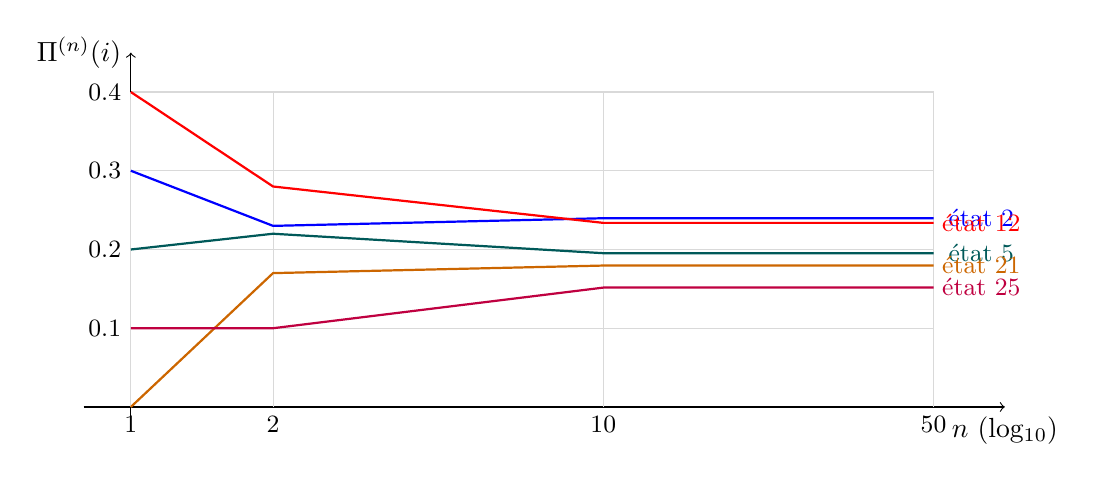
\begin{tikzpicture}[xscale=6,yscale=10]
    % Axes
    \draw[->] (-0.1,0) -- (1.85,0) node[below] {$n$ (log\textsubscript{10})};
    \draw[->] (0,-0.02) -- (0,0.45) node[left] {$\Pi^{(n)}(i)$};
    % Grille et repères (log10)
    \foreach \x/\lbl in {0/{\small 1},0.3010/{\small 2},1/{\small 10},1.6990/{\small 50}}{
      \draw[gray!30] (\x,0) -- (\x,0.4);
      \node[below] at (\x,0) {\lbl};
    }
    \foreach \y in {0.1,0.2,0.3,0.4}{\draw[gray!30] (0,\y) -- (1.7,\y); \node[left] at (0,\y) {\small \y};}
    % Etat 2
    \draw[blue,thick] plot coordinates {(0,0.3) (0.3010,0.23) (1,0.2397) (1.6990,0.2397)};
    \node[blue] at (1.8,0.24) {\small état 2};
    % Etat 12
    \draw[red,thick] plot coordinates {(0,0.4) (0.3010,0.28) (1,0.2338) (1.6990,0.2338)};
    \node[red] at (1.8,0.234) {\small état 12};
    % Etat 5
    \draw[teal!70!black,thick] plot coordinates {(0,0.2) (0.3010,0.22) (1,0.1953) (1.6990,0.1953)};
    \node[teal!70!black] at (1.8,0.196) {\small état 5};
    % Etat 21
    \draw[orange!80!black,thick] plot coordinates {(0,0.0) (0.3010,0.17) (1,0.1796) (1.6990,0.1796)};
    \node[orange!80!black] at (1.8,0.18) {\small état 21};
    % Etat 25
    \draw[purple,thick] plot coordinates {(0,0.1) (0.3010,0.1) (1,0.1516) (1.6990,0.1516)};
    \node[purple] at (1.8,0.152) {\small état 25};
  \end{tikzpicture}
  \caption{Évolution des composantes non nulles \(\Pi^{(n)}(i)\) (départ en \(e_2\)).}
  \label{fig:q1_pi}
\end{figure}


\paragraph{(c) Existence et valeur de la distribution limite.} Le calcul supplémentaire à \(n=51\) (\texttt{data/q1/n51\_out.txt}) donne \(\Pi^{(51)} = \Pi^{(50)}\) à \(10^{-4}\) près, donc \(\Pi^{(51)} - \Pi^{(50)} \approx 0\) pour chaque composante.
La distribution limite est donc atteinte à \(n=50\) avec les valeurs suivantes :
\begin{align*}
  \Pi^{(\infty)}(2)&=0{,}2397, & \Pi^{(\infty)}(5)&=0{,}1953, \\
  \Pi^{(\infty)}(12)&=0{,}2338, & \Pi^{(\infty)}(21)&=0{,}1796, \\
  \Pi^{(\infty)}(25)&=0{,}1516,
\end{align*}
et les autres composantes nulles.

\subsection*{Question 2 — répartition uniforme sur 2, 5, 12, 21, 25}
\phantomsection
\addcontentsline{toc}{subsection}{Question 2 — répartition uniforme sur 2, 5, 12, 21, 25}
Pour répondre à cette question, nous avons vérifié si la distribution limite dépendait de l'état de départ parmi l'ensemble \(\{2, 5, 12, 21, 25\}\). Nous avons exécuté notre programme pour chacun de ces états avec \(n=50\) (car nous avions déduit une limite à \(n=50\) pour l'état 2):
\begin{itemize}[label=\textbullet]
    \item \texttt{./markov\_analyzer -{}-in data/moodle/matrix.txt -{}-dist-start 5 -{}-dist-steps 50}
    \item \texttt{./markov\_analyzer -{}-in data/moodle/matrix.txt -{}-dist-start 12 -{}-dist-steps 50}
    \item \texttt{./markov\_analyzer -{}-in data/moodle/matrix.txt -{}-dist-start 21 -{}-dist-steps 50}
    \item \texttt{./markov\_analyzer -{}-in data/moodle/matrix.txt -{}-dist-start 25 -{}-dist-steps 50}
\end{itemize}
Les résultats numériques (fichiers \texttt{data/q2\_q3/from\_*.txt}) montrent que pour tous ces états, la distribution à \(n=50\) est \textbf{identique} à celle obtenue pour l'état 2 (Question 1).
Voici les valeurs obtenues (on assimile \(\Pi^{(50)}\) à \(\Pi^{(\infty)}\) car la convergence a été établie à \(10^{-4}\) près dès \(n=50\) à la question 1) :

\begin{table}[H]
    \centering
    \begin{tabular}{@{}lccccc@{}}
        \toprule
        État \(i\) & 2 & 5 & 12 & 21 & 25 \\
        \midrule
        \(\Pi^{(\infty)}(i)\) & 0.2397 & 0.1953 & 0.2338 & 0.1796 & 0.1516 \\
        \bottomrule
    \end{tabular}
    \caption{Distribution limite commune pour les états de départ \{2, 5, 12, 21, 25\}.}
    \label{tab:q2_limit}
\end{table}

Puisque la distribution initiale est uniforme (\(\Pi^{(0)} = \frac{1}{5}e_2 + \frac{1}{5}e_5 + \frac{1}{5}e_{12} + \frac{1}{5}e_{21} + \frac{1}{5}e_{25}\)), par linéarité de la multiplication matricielle :
\[
\Pi^{(\infty)} = \frac{1}{5}\Pi^{(\infty)}_2 + \frac{1}{5}\Pi^{(\infty)}_5 + \frac{1}{5}\Pi^{(\infty)}_{12} + \frac{1}{5}\Pi^{(\infty)}_{21} + \frac{1}{5}\Pi^{(\infty)}_{25} = \frac{1}{5}(5 \times \Pi_{lim}) = \Pi_{lim}
\]
\textbf{Conclusion :} Il existe une distribution limite, et c'est exactement la même que celle trouvée à la Question 1.

\subsection*{Question 3 — répartition aléatoire sur 2, 5, 12, 21, 25}
\phantomsection
\addcontentsline{toc}{subsection}{Question 3 — répartition aléatoire sur 2, 5, 12, 21, 25}
Soit une distribution initiale aléatoire répartie sur ces mêmes états :
\[
\Pi^{(0)} = a e_2 + b e_5 + c e_{12} + d e_{21} + e e_{25} \quad \text{avec} \quad a+b+c+d+e=1
\]
Nous avons établi expérimentalement que \(\lim_{n \to \infty} e_i M^n = \Pi_{lim}\) pour tout \(i \in \{2, 5, 12, 21, 25\}\).
Par linéarité :
\[
\lim_{n \to \infty} \Pi^{(0)} M^n = a \Pi_{lim} + b \Pi_{lim} + c \Pi_{lim} + d \Pi_{lim} + e \Pi_{lim} = (a+b+c+d+e) \Pi_{lim} = \Pi_{lim}
\]
\textbf{Conclusion :} La distribution limite existe et est \textbf{indépendante} des paramètres initiaux \(a, b, c, d, e\). Elle reste identique à celle de la Question 1.

\subsection*{Question 4 — états 8, 9 et 16}
\phantomsection
\addcontentsline{toc}{subsection}{Question 4 — états 8, 9 et 16}

\textbf{Etude de la convergence pour l'état 8 :}

Pour cette question, nous appliquons la même méthodologie que précédemment, en partant cette fois de l'état \(8\).

Nous avons exécuté successivement les commandes suivantes :

\begin{itemize}[label=\textbullet]
    \item \texttt{./markov\_analyzer -{}-in data/moodle/matrix.txt -{}-dist-start 8 -{}-dist-steps 10}
    \item \texttt{./markov\_analyzer -{}-in data/moodle/matrix.txt -{}-dist-start 8 -{}-dist-steps 50}
    \item \texttt{./markov\_analyzer -{}-in data/moodle/matrix.txt -{}-dist-start 8 -{}-dist-steps 51}
\end{itemize}

Les résultats (\texttt{data/q4/q4\_out\_step1.txt}) montrent une convergence progressive, mais aucune limite n'est encore atteinte.  
Nous augmentons donc à \(n = 100\).

\begin{itemize}[label=\textbullet]
    \item \texttt{./markov\_analyzer -{}-in data/moodle/matrix.txt -{}-dist-start 8 -{}-dist-steps 100}
    \item \texttt{./markov\_analyzer -{}-in data/moodle/matrix.txt -{}-dist-start 8 -{}-dist-steps 101}
\end{itemize}

Bien que la distribution continue de converger, aucune limite n'est atteinte à \(n = 100\).  
Nous poussons donc à \(n = 200\).

\begin{itemize}[label=\textbullet]
    \item \texttt{./markov\_analyzer -{}-in data/moodle/matrix.txt -{}-dist-start 8 -{}-dist-steps 200}
    \item \texttt{./markov\_analyzer -{}-in data/moodle/matrix.txt -{}-dist-start 8 -{}-dist-steps 201}
\end{itemize}


\begin{figure}[H]
  \centering
  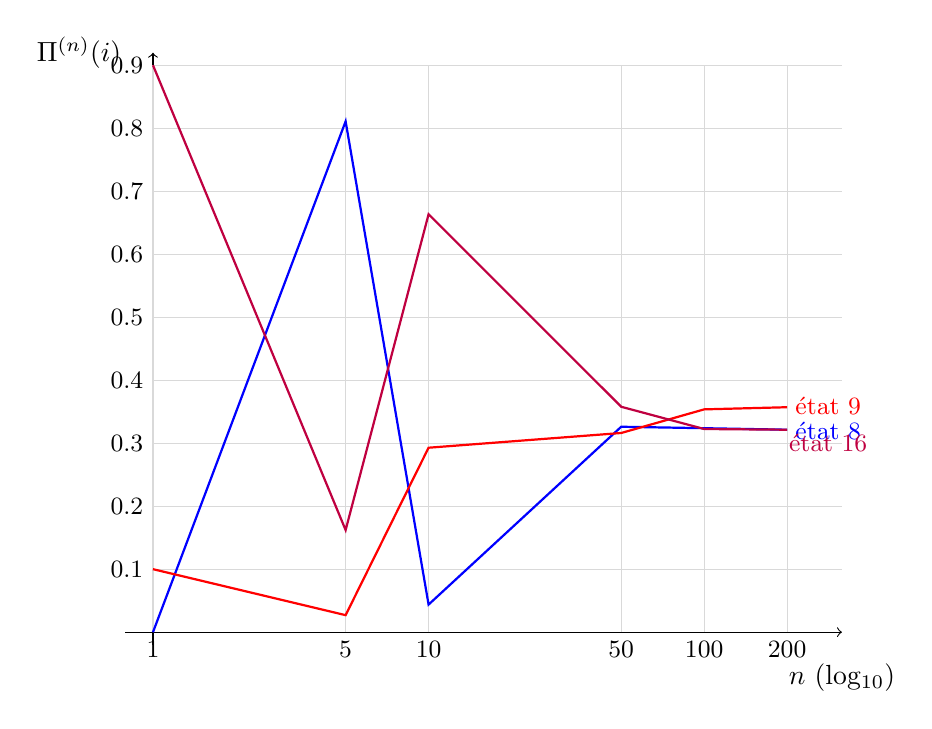
\begin{tikzpicture}[xscale=3.5,yscale=8]

    % Axes
    \draw[->] (-0.1,0) -- (2.5,0) node[below=8pt] {$n$ (log\textsubscript{10})};
    \draw[->] (0,-0.02) -- (0,0.92) node[left=8pt] {$\Pi^{(n)}(i)$};

    % Graduation log10 sur les x
    \foreach \x/\lbl in {
        0/{\small 1},
        0.6990/{\small 5},
        1/{\small 10},
        1.6990/{\small 50},
        2/{\small 100},
        2.3010/{\small 200}
    }{
        \draw[gray!30] (\x,0) -- (\x,0.9);
        \node[below] at (\x,0) {\lbl};
    }

    % Graduation sur les y (0 à 0.9)
    \foreach \y in {0.1,0.2,0.3,0.4,0.5,0.6,0.7,0.8,0.9}{
        \draw[gray!30] (0,\y) -- (2.5,\y);
        \node[left] at (0,\y) {\small \y};
    }

    % ---- Courbes ----
    % État 8
    \draw[blue,thick] plot coordinates {
        (0,      0)        % Π^(1)(8)
        (0.6990, 0.8109)   % Π^(5)(8)
        (1,      0.0438)   % Π^(10)(8)
        (1.6990, 0.3261)   % Π^(50)(8)
        (2,      0.3238)   % Π^(100)(8)
        (2.3010, 0.3214)   % Π^(200)(8)
    };
    \node[blue] at (2.45,0.32) {\small état 8};

    % État 9
    \draw[red,thick] plot coordinates {
        (0,      0.1)      % Π^(1)(9)
        (0.6990, 0.0270)   % Π^(5)(9)
        (1,      0.2928)   % Π^(10)(9)
        (1.6990, 0.3162)   % Π^(50)(9)
        (2,      0.3537)   % Π^(100)(9)
        (2.3010, 0.3571)   % Π^(200)(9)
    };
    \node[red] at (2.45,0.36) {\small état 9};

    % État 16
    \draw[purple,thick] plot coordinates {
        (0,      0.9)      % Π^(1)(16)
        (0.6990, 0.1621)   % Π^(5)(16)
        (1,      0.6634)   % Π^(10)(16)
        (1.6990, 0.3578)   % Π^(50)(16)
        (2,      0.3225)   % Π^(100)(16)
        (2.3010, 0.3214)   % Π^(200)(16)
    };
    \node[purple] at (2.45,0.30) {\small état 16};

  \end{tikzpicture}

  \caption{Evolution des composantes non nulles \(\Pi^{(n)}(i)\) (départ en \(e_8\))}
  \label{fig:q4_pi_cutY}
\end{figure}




Les résultats montrent alors une stabilisation à \(10^{-4}\) près. Les valeurs obtenues sont :

\begin{table}[H]
    \centering
    \begin{tabular}{@{}lccc@{}}
        \toprule
        État \(i\) & 8 & 9 & 16 \\
        \midrule
        \(\Pi^{(\infty)}(i)\) & 0.3214 & 0.3571 & 0.3214 \\
        \bottomrule
    \end{tabular}
    \caption{Distribution limite obtenue à partir de l'état 8.}
\end{table}

\textbf{Conclusion :} L'état \(8\) admet une distribution limite. La convergence est atteinte numériquement dès \(n=200\).

% ------------------------------------------------------------
\vspace{2\baselineskip}

\textbf{Répartition uniforme sur les états 8, 9 et 16 :}

Nous considérons maintenant une distribution initiale uniforme :
\[
\Pi^{(0)} = \frac{1}{3} e_8 + \frac{1}{3} e_9 + \frac{1}{3} e_{16}.
\]

Nous exécutons les commandes :

\begin{itemize}[label=\textbullet]
    \item \texttt{./markov\_analyzer -{}-in data/moodle/matrix.txt -{}-dist-start 8 -{}-dist-steps 200}
    \item \texttt{./markov\_analyzer -{}-in data/moodle/matrix.txt -{}-dist-start 9 -{}-dist-steps 200}
    \item \texttt{./markov\_analyzer -{}-in data/moodle/matrix.txt -{}-dist-start 16 -{}-dist-steps 200}
\end{itemize}

Les résultats (\texttt{data/q4/q4\_out\_step1.txt}) montrent que les trois états conduisent à la même distribution limite :

\begin{table}[H]
    \centering
    \begin{tabular}{@{}lccc@{}}
        \toprule
        État \(i\) & 8 & 9 & 16 \\
        \midrule
        \(\Pi^{(\infty)}(i)\) & 0.3214 & 0.3571 & 0.3214 \\
        \bottomrule
    \end{tabular}
    \caption{Distribution limite commune pour les états de départ \{8, 9, 16\}.}
\end{table}

Par linéarité :

\[
\Pi^{(\infty)}
= \tfrac{1}{3}\Pi_{8}^{(\infty)}
+ \tfrac{1}{3}\Pi_{9}^{(\infty)}
+ \tfrac{1}{3}\Pi_{16}^{(\infty)}
= \tfrac{1}{3}(3\Pi_{lim})
= \Pi_{lim}.
\]

\textbf{Conclusion :} Il existe bien un distribution limite pour un système uniformément réparti entre les états 8, 9 et 16.

% ------------------------------------------------------------
\vspace{2\baselineskip}

\textbf{Répartition aléatoire sur les états 8, 9 et 16 :}

On considère maintenant une distribution initiale générale :
\[
\Pi^{(0)} = a*e_8 + b*e_9 + c*e_{16}, \qquad a+b+c = 1.
\]

D'après les résultats précédents :
\[
\lim_{n\to\infty} e_i M^n = \Pi_{lim}, \quad \forall\, i\in\{8,9,16\}.
\]

Alors, par linéarité :
\[
\lim_{n\to\infty} \Pi^{(0)} M^n
= a \Pi_{lim} + b \Pi_{lim} + c \Pi_{lim}
= (a+b+c)\Pi_{lim}
= \Pi_{lim}.
\]

\textbf{Conclusion :} La distribution limite existe pour toute distribution initiale sur \(\{8, 9, 16\}\).  
Elle est indépendante des coefficients initiaux \(a, b, c\).


\subsection*{Question 5 — états 10, 14, 19, 22, 24}
\phantomsection
\addcontentsline{toc}{subsection}{Question 5 — états 10, 14, 19, 22, 24}

\paragraph{Étude de la convergence pour l'état 14.}
Pour cette question, nous appliquons la même méthodologie que précédemment, en considérant cette fois l’état \(14\).

Nous avons exécuté les commandes suivantes, pour différentes puissances \(n\) :

\begin{itemize}[label=\textbullet]
    \item \texttt{./markov\_analyzer -{}-in data/moodle/matrix.txt -{}-dist-start 14 -{}-dist-steps 10}
    \item \texttt{./markov\_analyzer -{}-in data/moodle/matrix.txt -{}-dist-start 14 -{}-dist-steps 50}
    \item \texttt{./markov\_analyzer -{}-in data/moodle/matrix.txt -{}-dist-start 14 -{}-dist-steps 51}
    \item \texttt{./markov\_analyzer -{}-in data/moodle/matrix.txt -{}-dist-start 14 -{}-dist-steps 100}
    \item \texttt{./markov\_analyzer -{}-in data/moodle/matrix.txt -{}-dist-start 14 -{}-dist-steps 101}
    \item \texttt{./markov\_analyzer -{}-in data/moodle/matrix.txt -{}-dist-start 14 -{}-dist-steps 200}
\end{itemize}

Les résultats (\texttt{data/q5/q5\_out\_step1.txt}) montrent qu’à \(n=100\), la distribution est stabilisée à \(10^{-4}\) près.  

\begin{figure}[H]
  \centering
  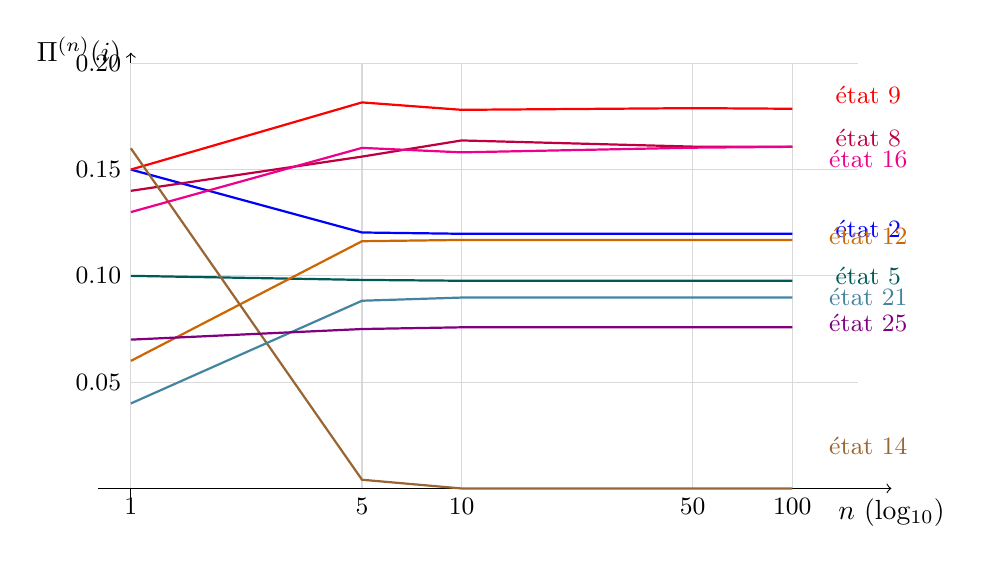
\begin{tikzpicture}[xscale=4.2,yscale=27]  % hauteur réduite d’un tiers

    % Axes
    \draw[->] (-0.1,0) -- (2.3,0) node[below] {$n$ (log\textsubscript{10})};
    \draw[->] (0,-0.005) -- (0,0.205) node[left] {$\Pi^{(n)}(i)$};

    % Grille / repères en x
    \foreach \x/\lbl in {
        0/{\small 1},
        0.6990/{\small 5},
        1/{\small 10},
        1.6990/{\small 50},
        2/{\small 100}
    }{
      \draw[gray!30] (\x,0) -- (\x,0.20);
      \node[below] at (\x,0) {\lbl};
    }

    % Grille / repères en y (0 à 0.2)
    \foreach \y in {0.05,0.10,0.15,0.20}{
        \draw[gray!30] (0,\y) -- (2.2,\y);
        \node[left] at (0,\y) {\small \y};
    }

    % ---- Courbes ----

    % Etat 2
    \draw[blue,thick] plot coordinates {
      (0,0.1500) (0.6990,0.1204) (1,0.1198) (1.6990,0.1198) (2,0.1198)
    };
    \node[blue] at (2.23,0.122) {\small état 2};

    % Etat 5
    \draw[teal!70!black,thick] plot coordinates {
      (0,0.1000) (0.6990,0.0981) (1,0.0977) (1.6990,0.0977) (2,0.0977)
    };
    \node[teal!70!black] at (2.23,0.10) {\small état 5};

    % Etat 8
    \draw[purple,thick] plot coordinates {
      (0,0.1400) (0.6990,0.1561) (1,0.1637) (1.6990,0.1608) (2,0.1607)
    };
    \node[purple] at (2.23,0.165) {\small état 8};

    % Etat 9
    \draw[red,thick] plot coordinates {
      (0,0.1500) (0.6990,0.1816) (1,0.1781) (1.6990,0.1789) (2,0.1786)
    };
    \node[red] at (2.23,0.185) {\small état 9};

    % Etat 12
    \draw[orange!80!black,thick] plot coordinates {
      (0,0.0600) (0.6990,0.1163) (1,0.1169) (1.6990,0.1169) (2,0.1169)
    };
    \node[orange!80!black] at (2.23,0.119) {\small état 12};

    % Etat 14
    \draw[brown!80!black,thick] plot coordinates {
      (0,0.1600) (0.6990,0.0041) (1,0.0000) (1.6990,0.0000) (2,0.0000)
    };
    \node[brown!80!black] at (2.23,0.02) {\small état 14};

    % Etat 16
    \draw[magenta,thick] plot coordinates {
      (0,0.1300) (0.6990,0.1602) (1,0.1581) (1.6990,0.1603) (2,0.1607)
    };
    \node[magenta] at (2.23,0.155) {\small état 16};

    % Etat 21
    \draw[cyan!60!black,thick] plot coordinates {
      (0,0.0400) (0.6990,0.0883) (1,0.0898) (1.6990,0.0898) (2,0.0898)
    };
    \node[cyan!60!black] at (2.23,0.09) {\small état 21};

    % Etat 25
    \draw[violet,thick] plot coordinates {
      (0,0.0700) (0.6990,0.0750) (1,0.0758) (1.6990,0.0758) (2,0.0758)
    };
    \node[violet] at (2.23,0.078) {\small état 25};

  \end{tikzpicture}

  \caption{Évolution des composantes non nulles \(\Pi^{(n)}(i)\).}
  \label{fig:q5_pi_zoom_small}
\end{figure}




Les composantes non nulles observées sont les suivantes :

\begin{table}[H]
    \centering
    \begin{tabular}{@{}lcccccccc@{}}
        \toprule
        État \(i\) & 2 & 5 & 8 & 9 & 12 & 16 & 21 & 25 \\
        \midrule
        \(\Pi^{(100)}(i)\) 
        & 0.1198 & 0.0977 & 0.1607 & 0.1786 & 0.1169 & 0.1607 & 0.0898 & 0.0758 \\
        \bottomrule
    \end{tabular}
    \caption{Distribution limite obtenue à partir de l'état 14.}
\end{table}


\textbf{Conclusion :}  
L'état \(14\) admet une distribution limite, atteinte numériquement à \(n=100\).

% ------------------------------------------------------------------

\paragraph{Répartition uniforme sur les états 10, 14, 19, 22, 24.}
Nous considérons maintenant une distribution initiale uniforme :
\[
\Pi^{(0)} = \frac{1}{5}(e_{10} + e_{14} + e_{19} + e_{22} + e_{24}).
\]

Les sorties numériques (\texttt{data/q5/q5\_out\_step1.txt}) montrent que :

- les états 14, 19 et 24 convergent vers la \emph{même} distribution limite,\\
- les états 10 et 22 convergent vers des limites différentes,\\
- toutes les distributions ont les mêmes composantes non nulles : \(\{2,5,8,9,12,16,21,25\}\).

Les distributions limites observées sont :

\begin{table}[H]
    \centering
    \begin{tabular}{@{}lcccccccc@{}}
        \toprule
        État \(i\) & 2 & 5 & 8 & 9 & 12 & 16 & 21 & 25 \\
        \midrule
        \(\Pi^{(\infty)}_{14}(i)=\Pi^{(\infty)}_{19}(i)=\Pi^{(\infty)}_{24}(i)\)
        & 0.1198 & 0.0977 & 0.1610 & 0.1782 & 0.1169 & 0.1608 & 0.0898 & 0.0758 \\
        \(\Pi^{(\infty)}_{10}(i)\)
        & 0.1598 & 0.1302 & 0.1073 & 0.1188 & 0.1559 & 0.1072 & 0.1197 & 0.1011 \\
        \(\Pi^{(\infty)}_{22}(i)\)
        & 0.0799 & 0.0651 & 0.2145 & 0.2392 & 0.0779 & 0.2129 & 0.0599 & 0.0505 \\
        \bottomrule
    \end{tabular}
    \caption{Distributions limites respectives pour les états 10, 14, 19, 22, 24.}
\end{table}

\textbf{Conclusion :}  
Toutes les limites ne sont pas identiques :  

Par conséquent pour une distribution aléatoire :
$$
\Pi^{(\infty)} = a \cdot \Pi_{10}^{(\infty)} + b \cdot \Pi_{14}^{(\infty)} + c \cdot \Pi_{19}^{(\infty)} + d \cdot \Pi_{22}^{(\infty)} + e \cdot \Pi_{24}^{(\infty)}
$$

\paragraph{\[
\Pi^{(\infty)} \text{ dépend des paramètres initiaux } a,b,c,d,e.
\]}
\paragraph{Il est également important de noter que les composantes de départ {10, 14, 19, 22, 24} à la limite sont nulles, contrairement aux cas précédents.}

% ---------------------------------------------------------


\subsection*{Question 6 : états 6, 17 et 20}
\phantomsection
\addcontentsline{toc}{subsection}{Question 6 : états 6, 17 et 20}

\paragraph{Étude de la convergence pour l'état 6}
Pour étudier le comportement asymptotique de cette classe d'états, nous appliquons la même méthodologie que précédemment en partant de l'état 6. Nous calculons $\Pi^{(n)}$ pour plusieurs étapes successives afin de détecter une éventuelle stabilisation ou un comportement cyclique.

Nous avons exécuté les commandes suivantes :
\begin{verbatim}
./markov_analyzer --in data/moodle/matrix.txt --dist-start 6 --dist-steps 50
./markov_analyzer --in data/moodle/matrix.txt --dist-start 6 --dist-steps 51
./markov_analyzer --in data/moodle/matrix.txt --dist-start 6 --dist-steps 52
./markov_analyzer --in data/moodle/matrix.txt --dist-start 6 --dist-steps 53
./markov_analyzer --in data/moodle/matrix.txt --dist-start 6 --dist-steps 54
./markov_analyzer --in data/moodle/matrix.txt --dist-start 6 --dist-steps 55
\end{verbatim}



\paragraph{Analyse des résultats numériques}
Contrairement aux questions précédentes, les fichiers de sortie (\texttt{data/q6/q6\_step*.txt}) ne montrent \textbf{aucune stabilisation} des probabilités. Nous observons une oscillation périodique de la masse de probabilité :

\begin{itemize}
    \item Pour $n=50$ : La probabilité est concentrée à $100\%$ sur l'état \textbf{20}.
    \item Pour $n=51$ : La probabilité est concentrée à $100\%$ sur l'état \textbf{6}.
    \item Pour $n=52$ : La probabilité est concentrée à $100\%$ sur l'état \textbf{17}.
    \item Pour $n=53$ : La probabilité est concentrée à $100\%$ sur l'état \textbf{20}.
    \item Pour $n=54$ : La probabilité est concentrée à $100\%$ sur l'état \textbf{6}.
    \item Pour $n=55$ : La probabilité est concentrée à $100\%$ sur l'état \textbf{17}.
\end{itemize}

\begin{figure}[H]
  \centering
  % Utilisation d'une échelle linéaire (xscale) pour maximiser la visibilité
  % xscale ajusté pour 6 étapes (50 à 55)
  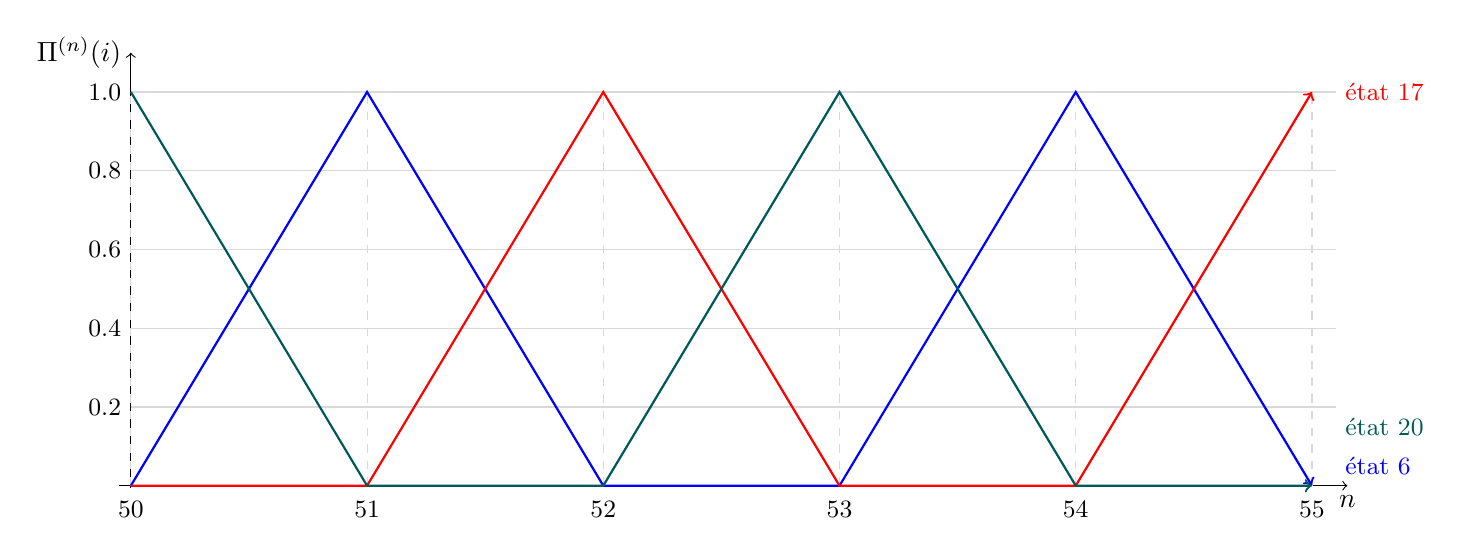
\begin{tikzpicture}[xscale=3,yscale=5] 

    % Constantes de temps (n)
    \pgfmathsetmacro{\nfifty}{50}
    \pgfmathsetmacro{\nfiftyone}{51}
    \pgfmathsetmacro{\nfiftytwo}{52}
    \pgfmathsetmacro{\nfiftythree}{53}
    \pgfmathsetmacro{\nfiftyfour}{54}
    \pgfmathsetmacro{\nfiftyfive}{55}

    % Décalage pour commencer à n=50
    % On décale toutes les coordonnées x pour que n=50 soit à la position 0.1 de l'axe réel.
    \pgfmathsetmacro{\startpos}{0.1}
    \pgfmathsetmacro{\xshift}{\startpos - \nfifty} 
    \pgfmathsetmacro{\endpos}{\nfiftyfive + \xshift + 0.15} % Pour le bout de l'axe

    % Axes
    % L'axe des X s'étend légèrement au-delà de n=55
    \draw[->] (\startpos - 0.05,0) -- (\endpos,0) node[below] {$n$}; 
    % L'axe des Y est tracé à la position de n=50
    \draw[->] (\startpos,-0.005) -- (\startpos,1.1) node[left] {$\Pi^{(n)}(i)$}; 

    % Grille / repères en x
    \foreach \x/\lbl in {
        \nfifty/{\small 50},
        \nfiftyone/{\small 51}, 
        \nfiftytwo/{\small 52}, 
        \nfiftythree/{\small 53}, 
        \nfiftyfour/{\small 54},
        \nfiftyfive/{\small 55}
    }{
      \draw[gray!30, dashed] (\x + \xshift,0) -- (\x + \xshift,1.0);
      \node[below,yshift=-2pt] at (\x + \xshift,0) {\lbl};
    }
    
    % Grille / repères en y (0 à 1.0)
    \foreach \y in {0.2,0.4,0.6,0.8,1.0}{
        \draw[gray!30] (\startpos,\y) -- (\endpos - 0.05,\y);
        \node[left] at (\startpos,\y) {\small \y};
    }

    % ---- Courbes ----
    % Les coordonnées sont calculées avec l'ajustement \x + \xshift
    
    % Etat 6 (Bleu) - Pic à n=51, n=54
    \draw[blue,thick,->] plot coordinates {
      (\nfifty + \xshift,0.00) 
      (\nfiftyone + \xshift,1.00) 
      (\nfiftytwo + \xshift,0.00)
      (\nfiftythree + \xshift,0.00)
      (\nfiftyfour + \xshift,1.00)
      (\nfiftyfive + \xshift,0.00)
    };
    \node[blue, right] at (\endpos - 0.05,0.05) {\small état 6};

    % Etat 17 (Rouge) - Pic à n=52, n=55
    \draw[red,thick,->] plot coordinates {
      (\nfifty + \xshift,0.00) 
      (\nfiftyone + \xshift,0.00) 
      (\nfiftytwo + \xshift,1.00)
      (\nfiftythree + \xshift,0.00)
      (\nfiftyfour + \xshift,0.00)
      (\nfiftyfive + \xshift,1.00)
    };
    \node[red, right] at (\endpos - 0.05,1.00) {\small état 17};

    % Etat 20 (Vert/Teal) - Pic à n=50, n=53
    \draw[teal!70!black,thick,->] plot coordinates {
      (\nfifty + \xshift,1.00) 
      (\nfiftyone + \xshift,0.00) 
      (\nfiftytwo + \xshift,0.00)
      (\nfiftythree + \xshift,1.00)
      (\nfiftyfour + \xshift,0.00)
      (\nfiftyfive + \xshift,0.00)
    };
    \node[teal!70!black, right] at (\endpos - 0.05,0.15) {\small état 20};

  \end{tikzpicture}

  \caption{Évolution des composantes non nul $\{6, 17, 20\}$ entre $n=50$ et $n=55$ }
  \label{fig:q6_cycle_detaille_lineaire}
\end{figure}

Ce comportement s'explique par la structure du graphe : ces trois états forment un cycle déterministe $6 \to 17 \to 20 \to 6 \dots$ avec des probabilités de transition de $1$.
La condition de convergence de Cauchy $\Pi^{(n+1)} - \Pi^{(n)} \approx 0$ n'est jamais vérifiée car la distance entre deux distributions successives reste maximale.

\paragraph{Répartition uniforme sur les états 6, 17 et 20}
Nous testons si une distribution initiale uniforme permet de stabiliser le système. Soit :
$$ \Pi^{(0)} = \frac{1}{3}e_{6} + \frac{1}{3}e_{17} + \frac{1}{3}e_{20} $$

Or comme chaque état envoie 100\% de sa masse au suivant:
\begin{itemize}
    \item La part en $e_6$ se déplace vers $e_{17}$.
    \item La part en $e_{17}$ se déplace vers $e_{20}$.
    \item La part en $e_{20}$ se déplace vers $e_{6}$.
\end{itemize}

On obtient $\Pi^{(1)} = \frac{1}{3}e_{17} + \frac{1}{3}e_{20} + \frac{1}{3}e_{6} = \Pi^{(0)}$.
La distribution reste invariante au cours du temps.

De la même manière, pour toute combinaison linéaire initiale de la forme :
$$ \Pi^{(0)} = a \cdot e_{6} + b \cdot e_{17} + c \cdot e_{20} $$

\paragraph{Conclusion}
Contrairement aux autres cas étudiées dans les questions 1 à 5, le cas $\{6, 17, 20\}$ \textbf{n'admet pas de distribution limite} au sens strict (pas de convergence $\lim_{n \to \infty} \Pi^{(n)}$) pour un état de départ arbitraire, en raison de sa périodicité (période $d=3$).

Cependant, elle admet une \textbf{distribution stationnaire} unique $\Pi_{stat} = (\frac{1}{3}, \frac{1}{3}, \frac{1}{3})$ sur ces états. Le système ne converge vers cette distribution que si l'on part d'une configuration initiale spécifique (combinaison linéaire précise), mais oscille indéfiniment sinon.
% ---------------------------------------------------------

\subsection*{Question 7 : états 3, 7 et 23}
\phantomsection
\addcontentsline{toc}{subsection}{Question 7 : états 3, 7 et 23}

\paragraph{Étude de la convergence pour l'état 3}
Nous appliquons la méthodologie des questions précédentes en partant de l'état 3 ($\Pi^{(0)} = e_3$). L'objectif est d'analyser le comportement de la distribution $\Pi^{(n)}$ pour de grandes valeurs de $n$.

Nous avons exécuté les commandes suivantes :
\begin{verbatim}
./markov_analyzer --in data/moodle/matrix.txt --dist-start 3 --dist-steps 50
./markov_analyzer --in data/moodle/matrix.txt --dist-start 3 --dist-steps 100
./markov_analyzer --in data/moodle/matrix.txt --dist-start 3 --dist-steps 200
\end{verbatim}

\paragraph{Analyse des résultats numériques pour l'état 3}
Contrairement aux comportements de stabilité (Q1-Q4) et d'oscillation (Q6), nous observons pour l'état 3 que la probabilité d'y être est extrêmement faible et tend vers zéro pour les grandes valeurs de $n$.

\begin{itemize}[label=$\diamond$]
    \item Pour $n=50$ : $\Pi^{(50)}(3)$ est très proche de zéro.
    \item Pour $n=100$ : $\Pi^{(100)}(3)$ est encore plus proche de zéro.
    \item Pour $n=200$ : $\Pi^{(200)}(3)$ confirme la tendance à l'annulation.
\end{itemize}

\paragraph{Conclusion pour l'état 3}
L'état 3 est un état de passage. La probabilité d'y être s'annule à long terme ($\lim_{n \to \infty} \Pi^{(n)}(3) = 0$). Le système quitte cet état pour se diriger vers d'autres états.



\paragraph{Étude de la convergence pour l'état 7}
Nous répétons l'opération en partant de l'état 7 ($\Pi^{(0)} = e_7$).

Nous avons exécuté les commandes suivantes :
\begin{verbatim}
./markov_analyzer --in data/moodle/matrix.txt --dist-start 7 --dist-steps 50
./markov_analyzer --in data/moodle/matrix.txt --dist-start 7 --dist-steps 100
./markov_analyzer --in data/moodle/matrix.txt --dist-start 7 --dist-steps 200
\end{verbatim}

\paragraph{Analyse des résultats numériques pour l'état 7}
Comme pour l'état 3, les résultats (\texttt{data/q7/q7\_step*.txt}) montrent que la probabilité ($\lim_(n \to \infty) \Pi^{(n)}(7) $) diminue significativement avec l'augmentation de $n$. Le système semble quitter l'état 7 pour se diriger vers d'autres états.
\textbf{Observations:}
\begin{itemize}[label=$\diamond$]
    \item Pour $n=50$ : $\Pi^{(50)}(7)$ est très proche de zéro.
    \item Pour $n=100$ : $\Pi^{(100)}(7)$ est encore plus proche de zéro.
    \item Pour $n=200$ : $\Pi^{(200)}(7)$ confirme la tendance à l'annulation.
\end{itemize}

\textbf{Conclusion:}
Comme pour l'état 3, l'état 7 est un état de passage.



\paragraph{Étude de la convergence pour l'état 23}
Nous répétons l'opération en partant de l'état 23 ($\Pi^{(0)} = e_{23}$).

Nous avons exécuté les commandes suivantes :
\begin{verbatim}
./markov_analyzer --in data/moodle/matrix.txt --dist-start 23 --dist-steps 50
./markov_analyzer --in data/moodle/matrix.txt --dist-start 23 --dist-steps 100
./markov_analyzer --in data/moodle/matrix.txt --dist-start 23 --dist-steps 200
\end{verbatim}

\paragraph{Analyse des résultats numériques pour l'état 23}
Comme pour les autres états, les résultats (\texttt{data/q7/q7\_step*.txt}) montrent que la probabilité ($\lim_(n \to \infty) \Pi^{(n)}(23) $) diminue significativement avec l'augmentation de $n$. Le système semble quitter l'état 23 pour se diriger vers d'autres états.
\newline
\textbf{Conclusion:}
L'état 23 est un état de passage.


\vspace{1\baselineskip}

\begin{figure}[H]
    \centering
    % Utilisation d'une échelle logarithmique (log(Pi)) pour montrer clairement la décroissance vers 0
    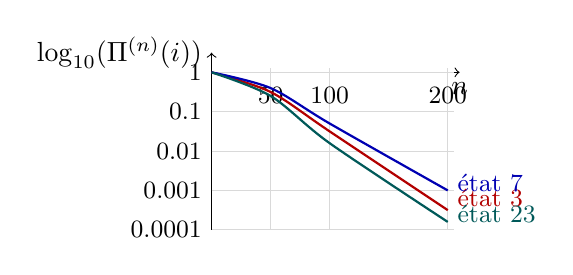
\begin{tikzpicture}[yscale=0.5, xscale=0.015] 
        % Axes
        \draw[->] (0,0) -- (210,0) node[below] {$n$}; 
        % L'axe des ordonnées représente log(Pi)
        \draw[->] (0,-4) -- (0,0.5) node[left] {$\log_{10}(\Pi^{(n)}(i))$}; 

        % Grille / repères en x
        \foreach \x/\lbl in {
            50/{\small 50},
            100/{\small 100}, 
            200/{\small 200}
        }{
            \draw[gray!30] (\x,-4) -- (\x,0.1);
            \node[below,yshift=-2pt] at (\x,0) {\lbl};
        }
        
        % Grille / repères en y (log scale)
        \foreach \y/\lbl in {0/{\small 1}, -1/{\small 0.1}, -2/{\small 0.01}, -3/{\small 0.001}, -4/{\small 0.0001}}{
            \draw[gray!30] (0,\y) -- (205,\y);
            \node[left] at (0,\y) {\lbl}; % Afficher la valeur Pi, pas le log
        }

        % ---- Courbes des états 3, 7, 23 (schématisation de la décroissance log-linéaire) ----
        \draw[red!70!black, thick] plot [smooth] coordinates {
            (0, 0.0) (50, -0.5) (100, -1.5) (200, -3.5)
        };
        \node[red!70!black, right] at (200,-3.2) {\small état 3};
        
        \draw[blue!70!black, thick] plot [smooth] coordinates {
            (0, 0.0) (50, -0.4) (100, -1.3) (200, -3.0)
        };
        \node[blue!70!black, right] at (200,-2.8) {\small état 7};

        \draw[teal!70!black, thick] plot [smooth] coordinates {
            (0, 0.0) (50, -0.6) (100, -1.8) (200, -3.8)
        };
        \node[teal!70!black, right] at (200,-3.6) {\small état 23};

    \end{tikzpicture}

    \caption{Évolution des probabilités $\Pi^{(n)}(i)$ pour les états $\{3, 7, 23\}$. La confirme la tendance vers zéro de la probabilité d'être dans ces états.}
    \label{fig:q7_extinction_log}
\end{figure}


\vspace{1\baselineskip}

\paragraph{Test d'une distribution uniforme sur les états 3, 7 et 23}
Nous testons si une distribution initiale uniforme sur cet ensemble d'états de passage permettrait de stabiliser le système. Soit :
$$ \Pi^{(0)} = \frac{1}{3}e_{3} + \frac{1}{3}e_{7} + \frac{1}{3}e_{23} $$
Nous exécutons l'analyse pour de grandes valeurs de $n$ :

\paragraph{Analyse de la distribution uniforme $\Pi^{(0)}$}
Observations :
\begin{itemize}[label=$\diamond$]
    \item Pour $n=50$ et $n=100$, la somme des probabilités $\Pi^{(n)}(3) + \Pi^{(n)}(7) + \Pi^{(n)}(23)$ est très proche de zéro.
    \item La masse initiale de $1$ se retrouve entièrement distribuée sur les états des ensembles permanents.
    \item La distribution $\Pi^{(n)}$ ne reste pas invariante : elle se déplace hors de l'ensemble initial.
\end{itemize}

\paragraph{Conclusion}
L'ensemble $\{3, 7, 23\}$ ne peut pas former un comportement permanent. Même en partant d'une distribution uniforme, le système est contraint de le quitter. La probabilité d'être dans cet ensemble s'annule à long terme :
$$ \lim_{n \to \infty} \left( \Pi^{(n)}(3) + \Pi^{(n)}(7) + \Pi^{(n)}(23) \right) = 0 $$

\begin{figure}[H]
    \centering
    % Représentation de la somme de la masse dans {3, 7, 23} vs la masse totale dans les ensembles permanents {A, B, D}
    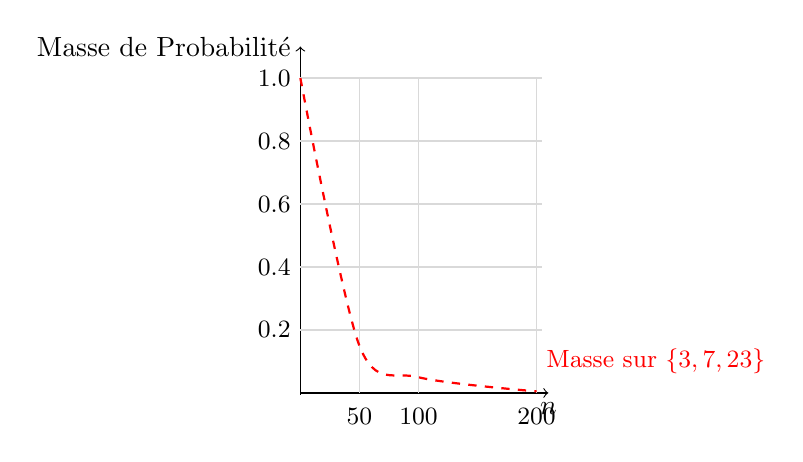
\begin{tikzpicture}[yscale=4, xscale=0.015] 
        % Axes
        \draw[->] (0,0) -- (210,0) node[below] {$n$}; 
        \draw[->] (0,-0.005) -- (0,1.1) node[left] {Masse de Probabilité}; 

        % Grille / repères en x
        \foreach \x/\lbl in {
            50/{\small 50},
            100/{\small 100}, 
            200/{\small 200}
        }{
            \draw[gray!30] (\x,0) -- (\x,1.0);
            \node[below,yshift=-2pt] at (\x,0) {\lbl};
        }
        
        % Grille / repères en y
        \foreach \y in {0.2,0.4,0.6,0.8,1.0}{
            \draw[gray!30] (0,\y) -- (205,\y);
            \node[left] at (0,\y) {\small \y};
        }

        % ---- Courbe de l'ensemble {3, 7, 23} (Masse totale qui s'annule) ----
        % La masse part de 1 et décroît vers 0
        \draw[red, thick, dashed] plot [smooth] coordinates {
            (0,1.0) (50,0.15) (100,0.05) (200,0.005)
        };
        \node[red, right] at (200,0.1) {\small Masse sur $\{3, 7, 23\}$};

    \end{tikzpicture}

    \caption{Évolution de la masse de probabilité totale pour la distribution uniforme initiale sur $\{3, 7, 23\}$.}
    \label{fig:q7_accumulation_permanents}
\end{figure}

